\section{Results}
\label{sec:results}

We first ask where the analysis time goes and how much of it the rewrite removes
(\S\ref{sec:anatomy}, \S\ref{sec:ladder}). We then ask when threads could help at all.
For the fork's thread pool to beat a single thread, four conditions must hold at once:
\begin{enumerate}
\item the metadata the lookups need must be \emph{cold}, or there is nothing to wait for
  (\S\ref{sec:fiemap}, \S\ref{sec:models});
\item the remaining device reads must be issued \emph{in the per-file part} that the
  threads share, not in the single tree walk that precedes it (\S\ref{sec:decompose});
\item a thread that waits must \emph{release the interpreter lock} (\S\ref{sec:gil});
\item the device must serve \emph{several requests at once} (\S\ref{sec:gil}).
\end{enumerate}
The fork's user-space \texttt{sleep} satisfies all four by construction. Real lookups
in FragPicker's workflow satisfy none of them in the common case, and we found no
configuration of the fork's code in which all four held.

\subsection{Where the analysis time goes}
\label{sec:anatomy}

\paragraph{Phase 1 costs about 70\,\textmu s per trace line.}
Figure~\ref{fig:phase1} times upstream's Phase~1 on its own (the first 61 lines of the
unmodified \texttt{processing.py}, cut programmatically) against the rewrite's
in-memory version, which writes the same files. On the WSL root file system the
upstream loop settles at 74\,\textmu s per line for long traces: 7.4\,s for
$10^5$ lines and 73.8\,s for $10^6$, against 0.32\,s and 2.4\,s for the rewrite. With
the working directory on ext4, XFS, Btrfs or F2FS it costs 68--79\,\textmu s per line
at $10^5$ lines, for one traced file or 1{,}000, so the file system hardly matters. A
system-call count explains it. For each trace line, Phase~1 makes about 41 calls: 30
one-byte \texttt{read}s, because upstream opens the trace with \texttt{buffering=0}
and then calls \texttt{readlines()}, which on an unbuffered file reads one byte at a
time, and then \texttt{openat}, \texttt{fstat}, an \texttt{ioctl} (the terminal check
of Python's \texttt{open}), five \texttt{lseek}s, one \texttt{write} and one
\texttt{close} to append a single line to \texttt{<inode>.txt}. The fork copied this
code into both of its paths.

\begin{figure}[t]
\centering
\figfile{width=\columnwidth}{../figs/e3_phase1_F1.pdf}
\caption{Phase~1 wall time against trace length, upstream versus rewrite, one traced
file. Medians of ten runs.}
\label{fig:phase1}
\end{figure}

\paragraph{Phase 2 and the rest of the pipeline cost fourteen processes per file.}
Table~\ref{tab:anatomy} (\S\ref{sec:background}) showed the per-file work. On the
real traces of E0, Table~\ref{tab:real} and Figure~\ref{fig:breakdown} split the whole
upstream pipeline into its steps. When a workload touches many files, the per-file steps
dominate. For \texttt{tar}, which read 5{,}100 files on the test file system, the
pipeline takes 165\,s: 97\,s in Phase~2, 56\,s in \texttt{hotness.sh} and 10\,s in
\texttt{merge.py}, against 1.7\,s in Phase~1. The rewrite does all three steps in
1.28\,s (129$\times$, 95\% CI 121--133). For \texttt{fio}'s 1{,}000 files the pipeline
takes 40.4\,s against 0.62\,s (65$\times$). When a workload touches one file, Phase~1
dominates instead: 83\% of the 0.75\,s for \texttt{read\_seq} and 92\% of the 8.6\,s
for \texttt{sqlite3}, whose trace has 160{,}935 lines (69\% of them for its database
file, the only traced file on the test file system). The
best \texttt{--parallel} setting makes
\texttt{processing.py} 7.4$\times$ faster than upstream on \texttt{tar} (13.4\,s against
98.7\,s) and 3.4$\times$ on \texttt{fio}, but slower than upstream on every one-file
trace (1.81\,s against 0.67\,s for \texttt{read\_seq}), because of its one-second floor
(\S\ref{sec:ladder}).

\begin{table*}[t]
\caption{Real traces, warm cache: wall time (s, median of seven runs) of upstream
\texttt{processing.py} (a), the best \texttt{--parallel} setting (d), the rewrite (c),
and of the whole pipeline (\texttt{processing.py}, \texttt{merge.py},
\texttt{hotness.sh}) against the rewrite doing all three steps.}
\label{tab:real}
\small
\centering
\inputtable{../results/tab_real.tex}
\end{table*}

\begin{figure*}[t]
\centering
\figfile{width=0.85\textwidth}{../figs/e2real_breakdown_warm.pdf}
\caption{Left: share of the upstream pipeline's time by step on each real trace. Right:
total time, upstream pipeline against the rewrite (median of seven runs, warm cache).}
\label{fig:breakdown}
\end{figure*}

\subsection{The ablation ladder}
\label{sec:ladder}

Figure~\ref{fig:ladder} runs every rung on synthetic traces of $F$ traced files, chosen
at random from a tree of $T = 10{,}000$ files of 16\,KB, 20 requests per file, with a
warm cache. All rungs produced identical output in every cell.

\begin{figure}[t]
\centering
\figfile{width=\columnwidth}{../figs/e2_vsF_ext4_T10000_warm_None.pdf}
\caption{Analysis wall time against the number of traced files $F$ ($T = 10{,}000$ files
in the tree, warm cache). Medians with 95\% bootstrap intervals; rungs as in
\S\ref{sec:method}.}
\label{fig:ladder}
\end{figure}

\paragraph{Upstream grows with $F \times T$.} Upstream costs about \textbf{[15]}\,ms per
traced file in this tree: one \texttt{find} over 10{,}000 entries plus a \texttt{sort}
and an \texttt{mv}. With 1{,}000 traced files it takes \textbf{[15.1]}\,s; the fork's
sequential path is the same code and the same time.

\paragraph{The parallel path has a floor of a second.} Every \texttt{--parallel} run
costs at least \textbf{[1.27]}\,s, even for one traced file, whatever the thread count.
Most of it is the resource-monitor thread that \texttt{processing.py} enables whenever
no dashboard is requested: it samples, sleeps for one second, and is joined only after
that sleep ends. The fork's own benchmark scripts turn monitoring off, so this cost
never appeared in its results.

\paragraph{The rewrite beats every thread count.} At $F = 1{,}000$ the rewrite takes
\textbf{[0.19]}\,s, \textbf{[80]}$\times$ faster than upstream and \textbf{[25]}$\times$
faster than the best parallel setting (\textbf{[4.76]}\,s with 8 threads). The parallel
path is faster than upstream only because its single walk replaces the per-file
\texttt{find}; it still starts two \texttt{sort} processes per file, one for the
discarded extents and one for the request file. Replacing the extent lookup with a stub
(rung e) saves 24\% at $F = 1{,}000$ (3.55\,s against 4.68\,s) and 7\% at $F = 10{,}000$
(34.3\,s against 36.7\,s): the lookups the threads were added to overlap are a minor
part of the parallel path's own time, which goes mostly to creating \texttt{sort}
processes. In McSherry et al.'s
terms~\cite{mcsherry2015cost}, the parallel engine's COST is unbounded: no thread count
we tried outperforms the single thread.

\subsection{What one extent lookup costs}
\label{sec:fiemap}

Table~\ref{tab:fiemap} times the fork's own lookup function (\texttt{stat},
\texttt{open}, FIEMAP, \texttt{close}) over files with a controlled number of extents
on four file systems, warm and cold, and counts the device reads per file. The extent
counts in the table are measured, not intended: our punch-and-rewrite procedure gave
exactly one extent per block on all four file systems.

\begin{table}[t]
\caption{Extent lookup per file (median of five passes over 100--1{,}000 files), and
device reads per file in a cold pass. One thread unless stated.}
\label{tab:fiemap}
\small
\inputtable{../results/tab_fiemap.tex}
\end{table}

\paragraph{Warm, it is microseconds.} With the cache warm, a lookup on ext4 or XFS
costs 16--25\,\textmu s for up to eight extents (30--44\,\textmu s on Btrfs) and grows
with the extent count, because the ioctl copies every extent out (about 0.6\,ms for
512 extents). This is the normal case for FragPicker: the analysis runs right after
the traced application has read these files, so their inodes and extent blocks are in
memory. F2FS is the exception: about 0.4\,ms per lookup even for one extent; we did
not find where that time goes.

\paragraph{Cold, the cost is the extent tree, not the inode.} With the cache cold,
files whose extents fit in the inode (four on ext4, more on XFS) still need almost no
device reads: 0.01 reads per file on ext4 and 0.04 on XFS, because inode-table
readahead brings in the inodes of hundreds of neighbouring files at once. Once the
extents spill into a tree block, every file needs one read of its own (1.0 per file
on both, two to three for 512 extents), and the lookup cost rises to 0.4--1.6\,ms on
our loop device. F2FS reads one block per file at every extent count, the file's
inode, which F2FS stores in a block of its own.

\paragraph{Threads helped only where the wait is outside FIEMAP.} On ext4 and XFS,
four and sixteen threads were \emph{slower} per file than one in every row
(0.21--0.96$\times$), even in the rows where each file needs its own device read. On
F2FS they were 1.4--1.6$\times$ faster in every row, and on Btrfs with 128 or more
extents 1.1--1.2$\times$. The difference matches where the wait happens: F2FS's one
read per file comes in through the \texttt{stat} and \texttt{open} calls, which release
the interpreter lock, while the read that remains on ext4 and XFS, the extent-tree
block, happens inside FIEMAP, where the fork's request keeps the lock held
(\S\ref{sec:gil}). We did not time the four calls separately, so this attribution is
an inference from the read counts.

\subsection{Three models of a slow device}
\label{sec:models}

Figure~\ref{fig:models} runs the code the fork benchmarked, its thread engine over
1{,}000 traced files plus the plain sequential loop its results file calls
``sequential'', under the three slow-device models of \S\ref{sec:method}, with a
5\,ms delay. Table~\ref{tab:models} gives the 1\,ms and 10\,ms cases.

\begin{figure*}[t]
\centering
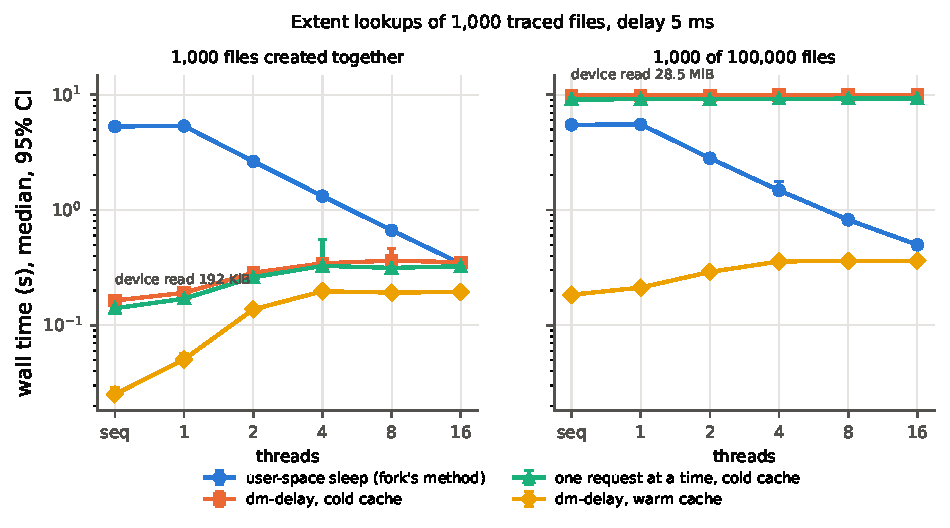
\includegraphics[width=0.9\textwidth]{../figs/e5_models_d5.pdf}
\caption{Wall time of the fork's extent-lookup engine against threads (``seq'': the
plain sequential loop) for 1{,}000 traced files, with a 5\,ms delay injected three
ways. Left: 1{,}000 files of 100\,KB created together; right: 1{,}000 files sampled
from a tree of 100{,}000. Medians of five runs with 95\% bootstrap intervals; the
labels give the data the device actually read in a cold run.}
\label{fig:models}
\end{figure*}

\paragraph{The user-space model reproduces the published speedup.} With
\texttt{time.sleep(0.005)} before every lookup, the sequential loop takes 5.31\,s and
16 threads take 0.343\,s, a speedup of 15.5$\times$ (95\% CI 14.3--15.7), close to the
fork's 12.74$\times$ (its sequential time, 7.28\,s, suggests a coarser sleep on that
machine). The model's prediction does not depend on the files at all: the scattered
case gives 11.0$\times$.

\paragraph{With the delay at the block layer, there is nothing to overlap.} When the
same 5\,ms is added to every read that reaches the device, the 1{,}000 files created
together are looked up in 0.164\,s from a cold cache by the sequential loop, 32 times
faster than the user-space model predicts, because the whole job reads only 192\,KiB
from the device: the directory blocks and a few inode-table blocks, each of which
holds the inodes of 16 files and is read ahead in groups of 32 blocks
(\texttt{inode\_readahead\_blks}, 32 on our kernel~\cite{kernelext4admin}), so one
miss brings in the inodes of 512 files.
Threads only add overhead (16 threads: 0.352\,s, 0.47$\times$). With a warm cache the
device is not touched at all and the sequential loop takes 25\,ms.

\paragraph{Scattered metadata is slow, but not in a way threads can fix.} When the
1{,}000 traced files are spread over a tree of 100{,}000, a cold run reads 28.5\,MiB
and takes 9.82\,s; but 16 threads take 9.99\,s, under dm-delay, which lets any number of
requests wait at once, and under the one-request-at-a-time device alike. Almost all of
the device time is spent before the threads start, in the single walk that builds the
inode map (\S\ref{sec:decompose}).

\begin{table}[t]
\caption{Speedup of 16 threads over the sequential loop (median, 95\% CI), and the
sequential loop's time, for each delay model. Five runs each.}
\label{tab:models}
\small
\input{../results/tab_models.tex}
\end{table}

\subsection{Where the cold reads happen}
\label{sec:decompose}

In the scattered case of Figure~\ref{fig:models} the device is busy, yet threads do not
help. Table~\ref{tab:decompose} splits a cold run into the tree walk that builds the
inode map and the per-file lookups that follow it, and counts device reads in each
part: \textbf{[E5b results pending]}.

\begin{table}[t]
\caption{A cold run of the scattered case split into the inode-map walk and the
per-file lookups (5\,ms configured delay), and the lookups alone when the paths are
already known. Medians of five runs.}
\label{tab:decompose}
\small
\inputtable{../results/tab_decompose.tex}
\end{table}

\subsection{The interpreter lock and the device}
\label{sec:gil}

Python threads overlap only while they are outside the interpreter: a blocking system
call releases the global interpreter lock (GIL) so that another thread can run. In
CPython 3.12.x and 3.13.x, \texttt{fcntl.ioctl} releases it only when it can copy the
argument into a 1{,}024-byte stack buffer. A larger writable buffer is passed to the
kernel in place, and the call runs with the GIL held (\texttt{fcntl\_ioctl\_impl} in
\texttt{Modules/fcntlmodule.c}, unchanged from v3.12.3 to v3.13.9; v3.14.0 releases
the GIL on this path, which we read in the source but did not run). The fork's FIEMAP
request has room for 32 extents, $32 + 32\cdot56 = 1{,}824$ bytes, so every FIEMAP call
holds the lock for as long as the kernel takes, including any device read for an
extent-tree block. The largest request that takes the releasing path holds 17 extents
(984 bytes).

Table~\ref{tab:gil} isolates the effect. Each of 200 files has 16 extents, so FIEMAP
must read one extent-tree leaf per file; before each timed pass we drop the caches and
\texttt{stat} every file, which brings the inodes in through readahead and leaves the
leaf blocks cold. Both request sizes return identical extents for every file, and every
pass reads 1.0 block per file from the device, so one thread takes the device's
latency per file (8.0\,ms under dm-delay, about 6\,ms on NBD; \S\ref{sec:method}).

When the device serves many requests at once (dm-delay, or NBD with 32 server
threads), 16 threads finish the 984-byte requests 14.6$\times$ and 14.9$\times$ faster
than one thread, but the 1{,}824-byte requests, ours or the fork's own
\texttt{FiemapAnalyzer}, gain nothing: 1.00$\times$ on both devices. Sixteen processes
issuing the same 1{,}824-byte requests gain 15.0$\times$ and 14.9$\times$, so the
request size matters only because of the lock. On the device that serves one request at
a time, nothing gains more than 1.09$\times$. The fork's process engine reaches
8.1$\times$ and 7.8$\times$; its 16 workers take about 0.1\,s longer than ours, which we
did not investigate. With no delay, the fork's thread pool is slower than one thread
(0.107\,s against 0.076\,s).

\begin{table}[t]
\caption{Speedup of 16 workers over one for FIEMAP calls that each wait for one device
read, by request size, threads or processes, and device. Median of five passes, 95\%
bootstrap interval.}
\label{tab:gil}
\small
\inputtable{../results/tab_gil.tex}
\end{table}

Two consequences follow. First, the condition the fork needs most, that waits overlap,
fails exactly for the files FragPicker exists to fix: the fragmented ones, whose
extents do not fit in the inode. Second, the user-space delay hid this as well,
because \texttt{time.sleep} releases the GIL and runs before the ioctl. The fork's
process engine would overlap the waits, but \texttt{--parallel} does not use it, and it
would overlap work that the analysis does not need (\S\ref{sec:correct}).

% Real slow device (E6): pending the owner's hardware or a cloud HDD instance.
% If E6 is not run, this file stays empty and the threats section says so.

